\subsubsection{Pruebas del módulo de procesado digital de señal}

Para probar el módulo de procesado digital de señal, se conecta un generador de señal a la entrada del \texttt{ADC} de la placa y se mide la salida del \texttt{DAC} mediante un osciloscopio.

Primero probamos si el túnel de audio funciona, para lo cual no habilitamos ningún filtro. Como se ve en la \autoref{fig:4-1-dsp-directo}, se tiene exactamente la misma señal pero retrasada unos milisegundos.

\begin{figure}[h]
    \centering
    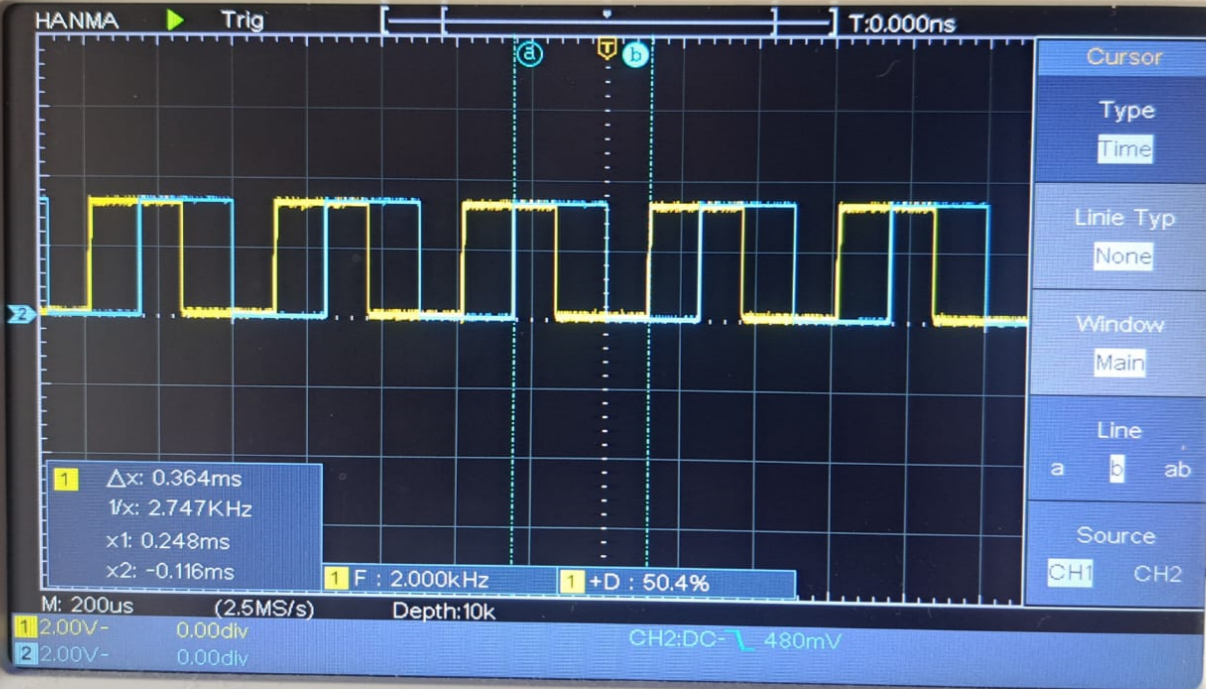
\includegraphics[width=0.5\textwidth]{images/4/4-1/audio-directo.png}
    \caption{Camino de audio sin procesado}
    \label{fig:4-1-dsp-directo}
\end{figure}

Después, probamos por ejemplo a reducir las altas frecuencias y bajar un poco el volumen, obteniendo una salida como la de la \autoref{fig:4-1-dsp-procesado}.

\begin{figure}[h]
    \centering
    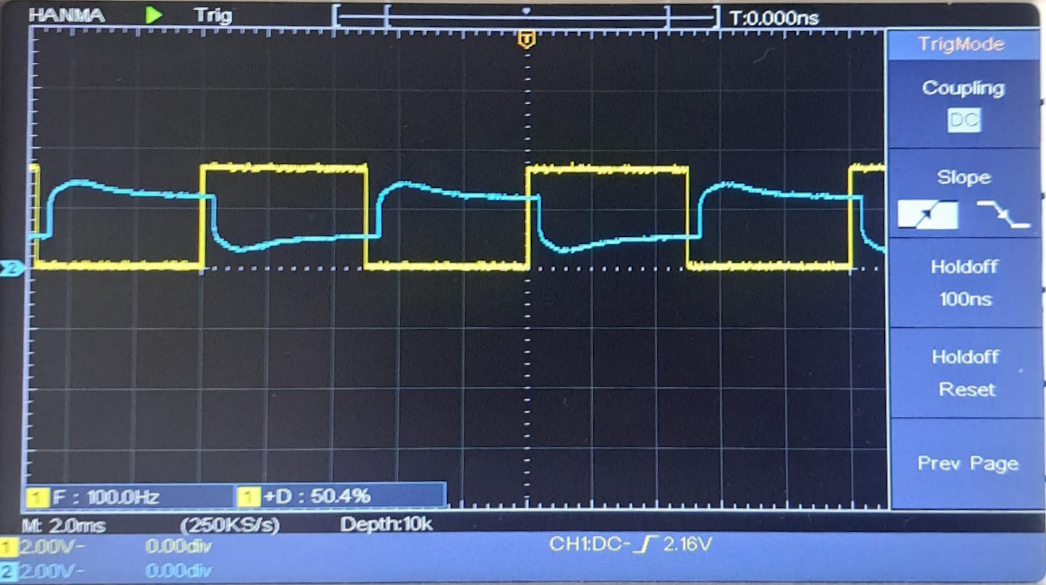
\includegraphics[width=0.5\textwidth]{images/4/4-1/audio-procesado.png}
    \caption{Señal cuadrada procesada digitalmente}
    \label{fig:4-1-dsp-procesado}
\end{figure}